\documentclass{sigchi}

% Use this command to override the default ACM copyright statement (e.g. for preprints). 
% Consult the conference website for the camera-ready copyright statement.


%% EXAMPLE BEGIN -- HOW TO OVERRIDE THE DEFAULT COPYRIGHT STRIP -- (July 22, 2013 - Paul Baumann)
% \toappear{Permission to make digital or hard copies of all or part of this work for personal or classroom use is 	granted without fee provided that copies are not made or distributed for profit or commercial advantage and that copies bear this notice and the full citation on the first page. Copyrights for components of this work owned by others than ACM must be honored. Abstracting with credit is permitted. To copy otherwise, or republish, to post on servers or to redistribute to lists, requires prior specific permission and/or a fee. Request permissions from permissions@acm.org. \\
% {\emph{CHI'14}}, April 26--May 1, 2014, Toronto, Canada. \\
% Copyright \copyright~2014 ACM ISBN/14/04...\$15.00. \\
% DOI string from ACM form confirmation}
%% EXAMPLE END -- HOW TO OVERRIDE THE DEFAULT COPYRIGHT STRIP -- (July 22, 2013 - Paul Baumann)


% Arabic page numbers for submission. 
% Remove this line to eliminate page numbers for the camera ready copy
\pagenumbering{arabic}

% Load basic packages
\usepackage{tabularx} 
\usepackage{balance}  % to better equalize the last page
\usepackage{graphics} % for EPS, load graphicx instead
\usepackage{times}    % comment if you want LaTeX's default font
\usepackage{url}      % llt: nicely formatted URLs

% llt: Define a global style for URLs, rather that the default one
\makeatletter
\def\url@leostyle{%
  \@ifundefined{selectfont}{\def\UrlFont{\sf}}{\def\UrlFont{\small\bf\ttfamily}}}
\makeatother
\urlstyle{leo}


% To make various LaTeX processors do the right thing with page size.
\def\pprw{8.5in}
\def\pprh{11in}
\special{papersize=\pprw,\pprh}
\setlength{\paperwidth}{\pprw}
\setlength{\paperheight}{\pprh}
\setlength{\pdfpagewidth}{\pprw}
\setlength{\pdfpageheight}{\pprh}

% Make sure hyperref comes last of your loaded packages, 
% to give it a fighting chance of not being over-written, 
% since its job is to redefine many LaTeX commands.
\usepackage[pdftex]{hyperref}
\hypersetup{
pdftitle={SIGCHI Conference Proceedings Format},
pdfauthor={LaTeX},
pdfkeywords={SIGCHI, proceedings, archival format},
bookmarksnumbered,
pdfstartview={FitH},
colorlinks,
citecolor=black,
filecolor=black,
linkcolor=black,
urlcolor=black,
breaklinks=true,
}

% create a shortcut to typeset table headings
\newcommand\tabhead[1]{\small\textbf{#1}}

% shortcut for stakeholder table
\newcommand{\stakeholdertable}{
\begin{table*}
  \centering
  	\begin{tabularx}{0.9\textwidth}{|X|X|X|X|}
    \hline
    \tabhead{Direct Stakeholders} & \tabhead{Benefits/Harms} & \tabhead{Values} & \tabhead{Conflicts} \\
    \hline
    System managers & 
		\underline{Benefits}: Able to fix problems more quickly\newline
		\underline{Benefit or harm}: Less time doing maintenance and tending plants by hand\newline
		\underline{Harm}: Could be alerted of emergencies at any time
	&	Human welfare\newline
	 	Autonomy\newline
		Calmness\newline
		Free time away from work\newline
		Interaction with nature\newline
		Physical interaction with systems\newline
		Awareness (of system functioning)
	& Physical interaction with systems and awareness may conflict with calmness and free time away from work \\
%    \hline
%	Owners of system &
%		\underline{Benefits}: System reduces labor and maintenance costs\newline
%		Produce organic and high quality food\newline
%		\underline{Harms}: Could suffer financial loss if system breaks down
%	&	Ownership and property\newline 
%		Efficiency 
%	& \\
%    \hline
    \hline
    \tabhead{Indirect Stakeholders} & \tabhead{Benefits/Harms} & \tabhead{Values} & \tabhead{Conflicts} \\
    \hline
    Restaurants and\newline restaurant customers &
		\underline{Benefits}: Know about where their food comes from\newline
		Provide feedbacks or improvements to owner\newline
		\underline{Harms}: Could be lied to if presented with false information
	&	Trust\newline
		Accountability\newline
		Environmental sustainability\newline
		Autonomy\newline
		Ownership and property (restaurants)
	&	Ownership and property (in the form of profitability) may compete with environmental sustainability\\
    \hline
  \end{tabularx}
  \caption{Paired down list of stakeholders}
  \label{tab:stakeholders}
\end{table*}}

\newcommand{\tasktable}{
\begin{table}
\centering
\begin{tabularx}{0.45\textwidth}{|X|X|X|X|}
    \hline
    \tabhead{Task instruction} & \tabhead{Feature tested} \\
    \hline
    Identify whether any feeds are currently outside of optimal limits. & The default view of the chart, whether optimal settings zone is clear \\
    \hline
    Find how many times the feeds went outside optimal parameters in the last 3 months. & Whether brush (timeline) has correct affordances\\
    \hline
    Find out if/how many times each feed went outside optimal settings between March and February. & Whether people view all settings at once, or use the buttons to view them individually; requires additional use of brush\\
    \hline
\end{tabularx}
  \caption{Tasks used to test interface prototype}
  \label{tab:tasks}
\end{table}
}

% End of preamble. Here it comes the document.
\begin{document}

\title{Developing an Aquaponics Interface}

\numberofauthors{3}
\author{
  \alignauthor Justin Bare\\
    \affaddr{University of Washington}\\
    \email{jbare@cs.washington.edu}\\
  \alignauthor Laurel Hart\\
    \affaddr{University of Washington}\\
    \email{hart1a@uw.edu}\\
  \alignauthor Sam Wilson\\
    \affaddr{University of Washington}\\
    \email{samw11@cs.washington.edu}\\
}

\maketitle

\begin{abstract}
Aquaponics is a method of farming which can be useful in an urban setting for sustainably producing food and increasing food security. This study pursued two goals related to the display of aquaponics system information: to extend the abilities of managers to operate such systems effectively and to provide environmentally conscious customers with relevant information about the sustainability of the system. By using value sensitive design, we produced an interface for monitoring an aquaponics system and provide suggestions for furnishing interested parties with sustainability information.
\end{abstract}

\keywords{Aquaponics; sustainability; value sensitive design;}

\category{H.5.2.}{Information Interfaces and Presentation}{User Interfaces}

\section{Introduction}

Aquaponics is a method of farming which produces fish and vegetables simultaneously in the same system (see Figure~\ref{fig:skales}). It is particularly useful for increasing food security and producing food sustainably in urban settings. Aquaponics systems are very modular and easy to maintain once they have been set up and equipped with automated monitoring and control devices. With only a few parameters to check every day, even large systems can be managed well by a single person with the right tools. 

The intent of this project is two-fold: to extend the abilities of managers to operate their aquaponics systems effectively and to provide environmentally conscious customers with relevant information about the sustainability of the system. To do this, the project will follow a value sensitive design approach.

\begin{figure*}
\centering
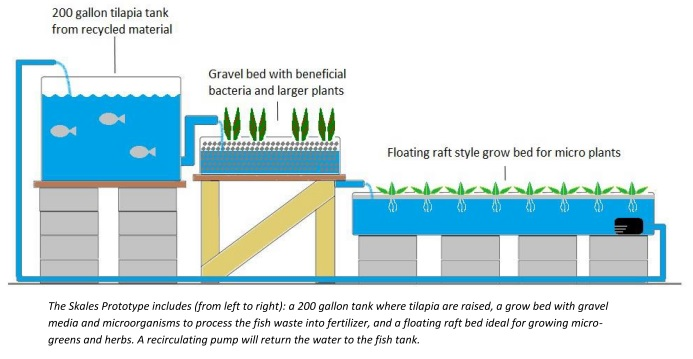
\includegraphics[width=0.9\textwidth]{systemDiagram}
\caption{Skales Cooperative aquaponics system}
\label{fig:skales}
\end{figure*}

\section{Related Work}
\subsubsection{Aquaponics}

As Domingues et. al. demonstrate in \cite{automated}, computer automation of the hydroponic growing process is very effective for increasing efficiency and reducing labor. The current project aims to implement this type of automation for aquaponics systems, which are somewhat similar to hydroponic systems. However, there appears to be a lack of research into the human factors of the design of such an automation system. Based on the interviews with experts in this project, urban aquaponics growers have specific needs for novel features of an interface that would allow them to interact with their systems remotely. The current project has a direct goal of incorporating the values of these experts into the design of an effective online interface for aquaponics systems. 

There is prior work \cite{smallBusiness, cueing} in engaging consumers in thinking about the sustainability of their actions, and also in engaging companies in analyzing the sustainability of their operations \cite{smallBusiness, audit}. Salv\'a et. al. identify several key factors of sustainability that companies and consumers are interested in. Cornelissen et. al. have determined effective ways for engaging people positively in environmental behaviors. Bonanni et. al. have studied a specific tool which allows businesses to present information to customers about the amount of shipping used to produce their products. The current project aims to combine and expand on these three pieces of work. Specifically, there will be a customer interface showing real time sustainability information (based directly off of the sensor readings) about the operations of the aquaponics system. Customers will be able to see details about water, energy, waste, etc. and how the measures of these sustainability factors compare to the average American farm. The design of the customer interface for a positive experience with environmentally friendly behavior will be well informed by the values of consumers, as determined through surveys, interviews, and other studies. 

In general there seems to be a lack of research into design of well integrated computing technologies for sustainable urban food production and consumption, so this project will be an important step in seeding this area of research in the HCI community. Furthermore, it should demonstrate a helpful addition to the farm-to-table movement by introducing real sustainability information that is available for the consumer to see how their specific actions, in their specific location, benefit the environment, as opposed to generalizing about the environmental benefits of farm-to-table, which can vary significantly from place to place.

\subsubsection{Value Sensitive Design}
We have alluded several times to the idea of incorporating values into our design. In ~\cite{VSD}, a theoretically grounded approach called Value Sensitive Design (VSD) is outlined so that researchers can use it to formally account for human values in the design process. This approach goes beyond previous approaches which explored design for specific values, like privacy or autonomy. Since we perceived that our system would benefit from supporting several  different values beyond the obvious one of sustainability, we determined that VSD was critical to our work. 
% \cite{moreVSD}

\section{Methods}

Our project began with brainstorming possible stakeholders in the design of the system, followed by hypothesizing about possible benefits and harms they would encounter as a result of the system, and then synthesizing these to come up with values to design for and conflicts between values of stakeholders. This was then further investigated using semi-structured interviews to weigh the importance of various values in order to guide our design process. We also discovered several specific design features to include through the interviews. Then, we moved on to actually designing the interface and testing it with users. The details of these procedures are described in the following sections:

\subsection{Identifying stakeholders}

Our first step was to create a list of potential stakeholders. Although our list was initially quite extensive, we chose to focus on a few principle ones in our investigation (see Table~\ref{tab:stakeholders}). In particular, we chose system managers and restaurants owners/customers because we suspected their needs could be addressed using the system monitoring information available to us. Once we identified these two key groups, we began by constructing surveys in order to investigate the values of each. In response to feedback about our plan of investigation, the surveys were adapted into outlines for semi-structured interviews. We had identified some values for each group in the initial step of identifying stakeholders, but needed to verify whether our intuitions were accurate. From this point, our investigations of the key groups diverged, and are addressed individually below. 
\stakeholdertable

\subsubsection{Direct Stakeholders}

The direct stakeholders, or system managers, can also be considered the ``expert users'' of our interface, whose needs and skills are specifically adapted to the system at hand. Our informal interviews allowed us to identify a few key parameters that needed to be monitored using the interface: pH balance, water temperature, nitrogen levels, air temperature, and dissolved oxygen. Ideally the system managers would be able to add any type of parameter that could be monitored, allowing for extensible use. The system managers also stated a preference for all data to be visible on one graph, rather than a separate graph for each parameter. The interviews also confirmed the conflict between valuing calmness and free time away from the system versus physical interaction with and awareness of the system; system managers stated that an online interface would drastically improve maintenance, but that alerts would need to be immediate and disruptive if urgent. 

Based on these preference statements, we outlined a few key features:
\begin{itemize}
\item An adustable timeline, which would allow system operators to not only see up-to-date data, but also arbitrary intervals of time in order to look for trends in the system's performance. 
\item Multiple visualizations of live system data. A line graph works well for data over time, but under-emphasizes the time frame a system manager will most often be concerned about when checking the site: the present moment. The system will also eventually be fitted with a camera to allow the system manager to monitor data that perhaps is not best represented by numbers, such as fish activity. 
\item Individual, customizable settings for each parameter. Each parameter has its own value range. Also true is that each parameter has a particular range that it should stay within for best performance of the system; the system manager should be able to set that range for each parameter. 
\item A normalized view of all parameters. Because each parameter has its own value range, the request that they all be displayed on one graph was at first conceptually daunting. Since each parameter also has a particular range that it should stay within, we therefore conceptualized this as an ``optimal zone'' by which to normalize. 
\item The ability to add parameters as more monitoring equipment becomes available. 
\end{itemize}

Based on these features, we produced our first sketches (Figures~\ref{fig:sketch1} and \ref{fig:sketch2}). 
\begin{figure}[!h]
\centering
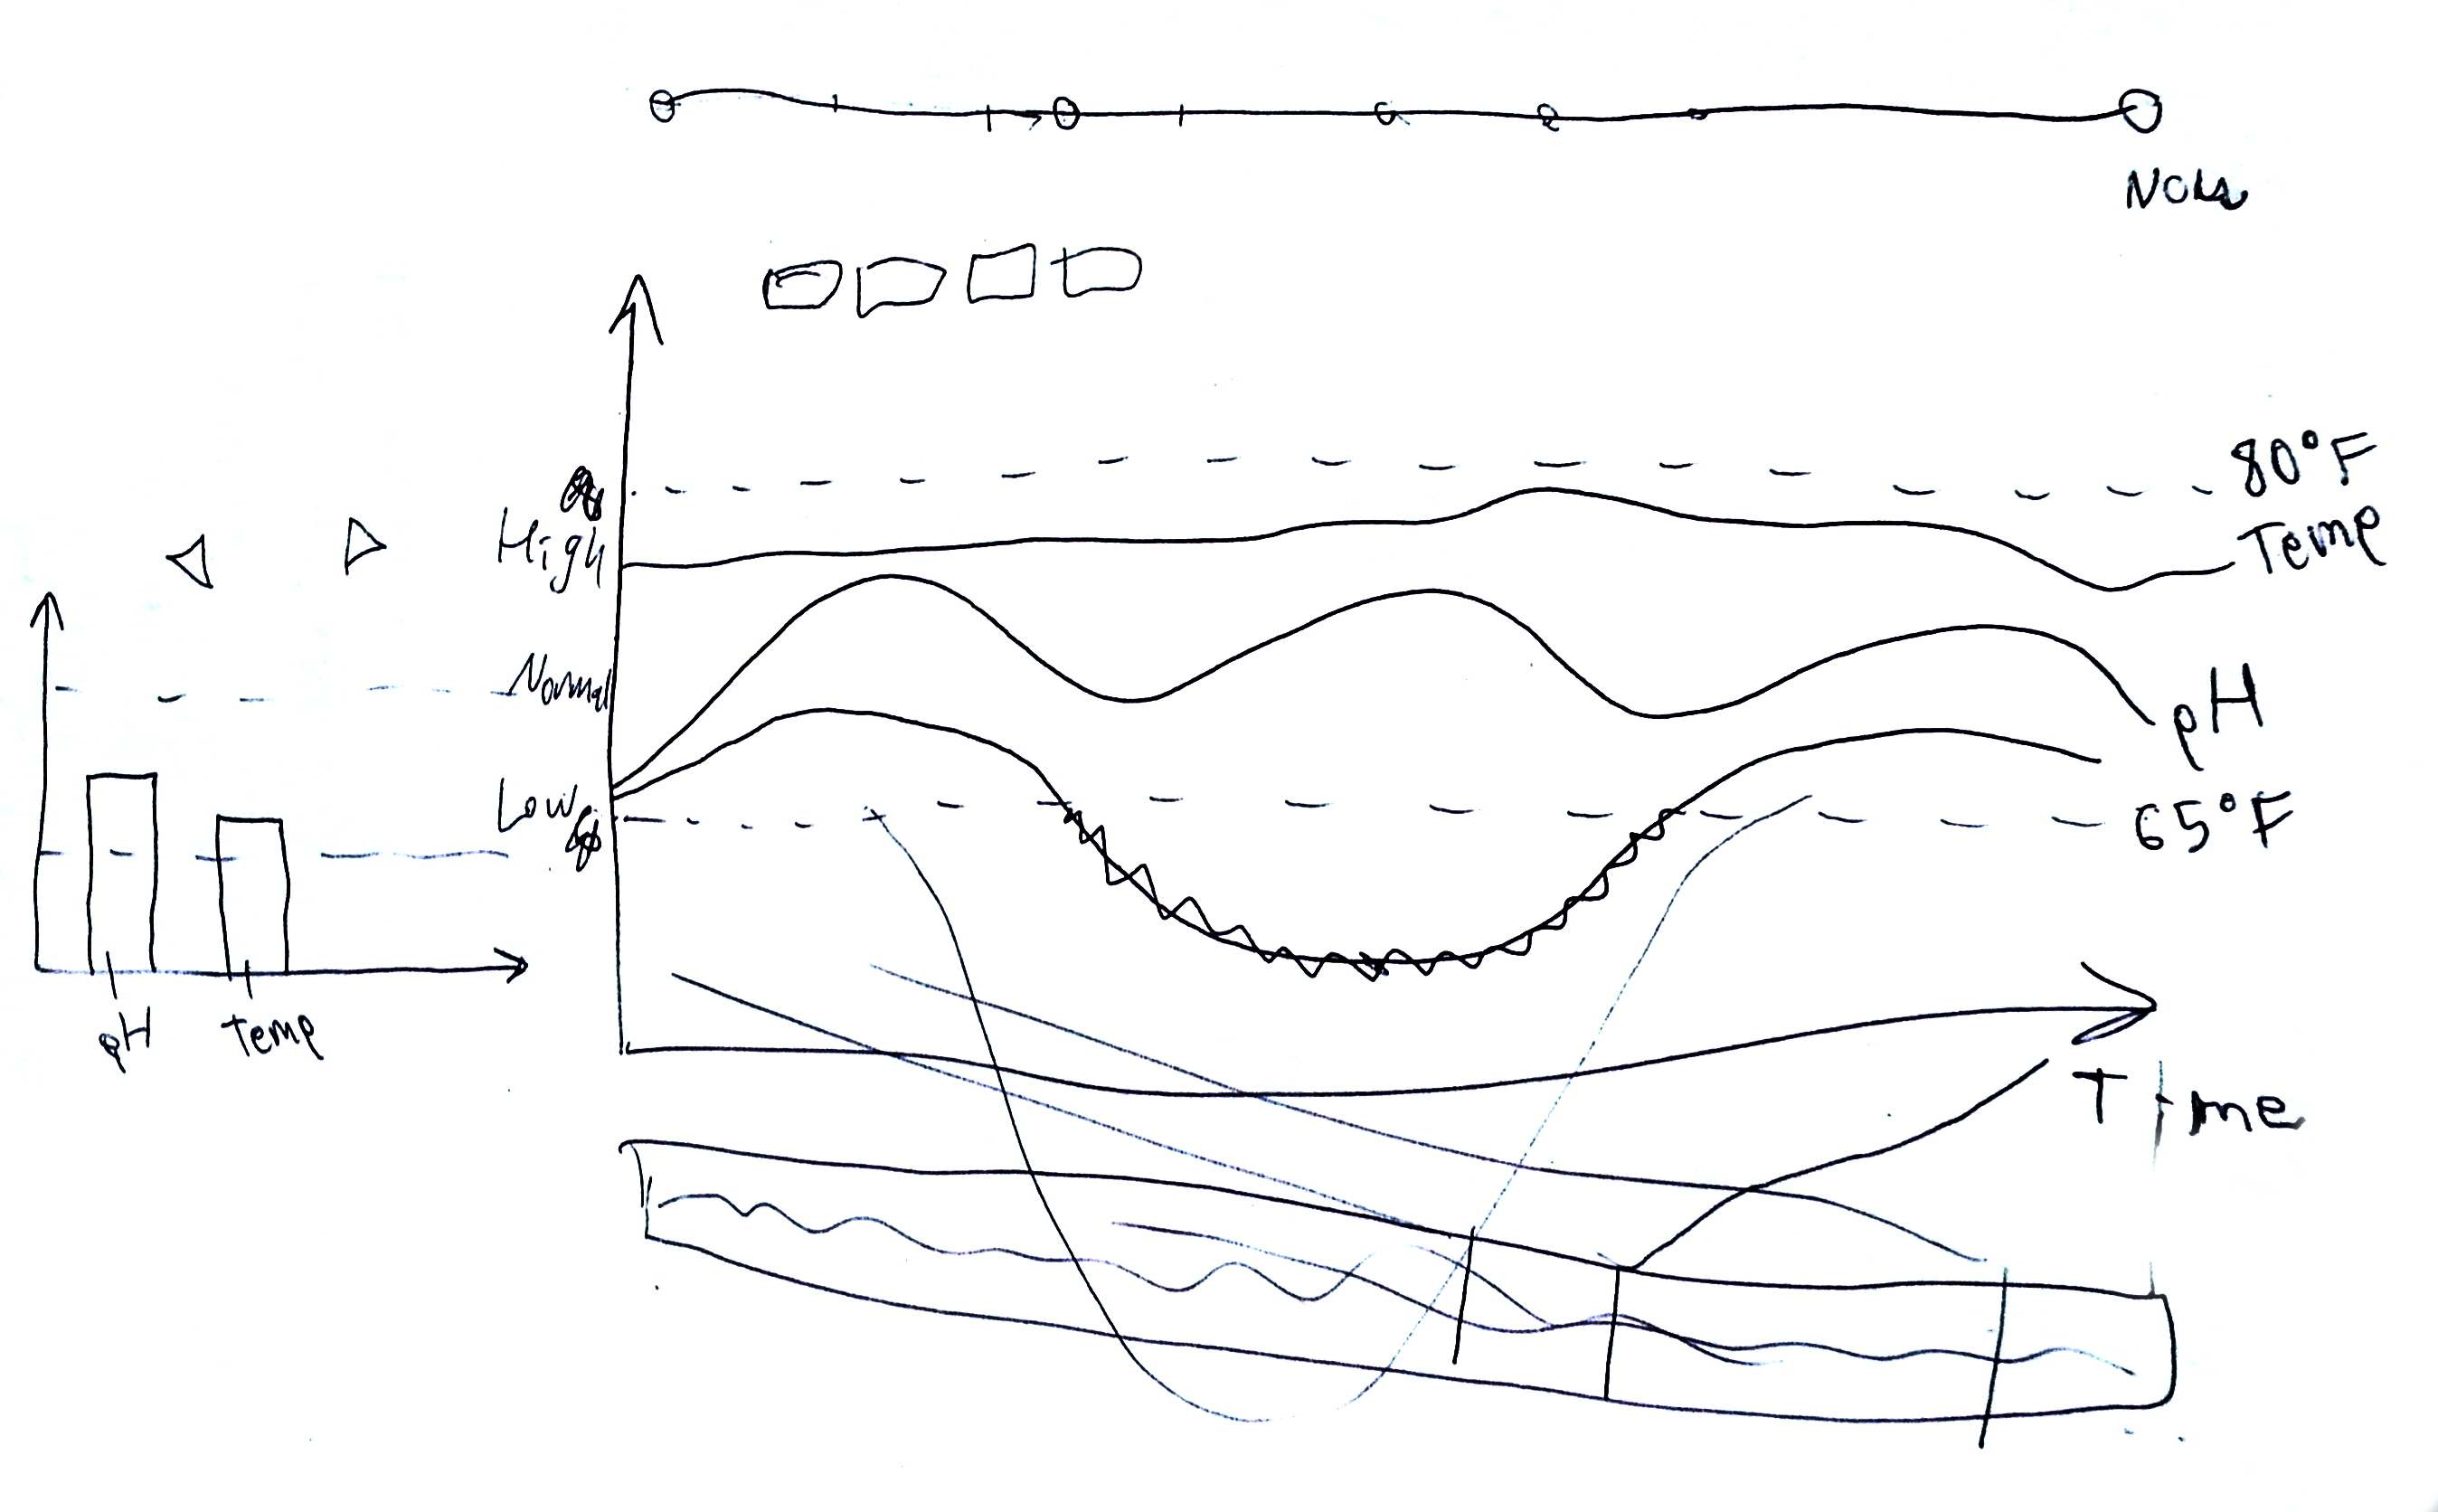
\includegraphics[width=0.9\columnwidth]{Sketch1}
\caption{Initial sketch in response to system manager's desire to see all information at a glance.}
\label{fig:sketch1}
\end{figure}
\begin{figure}[!h]
\centering
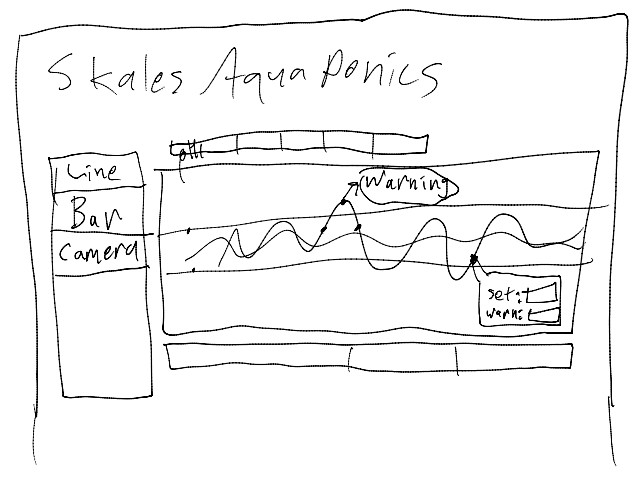
\includegraphics[width=0.9\columnwidth]{Sketch2}
\caption{Refinement upon first sketch.}
\label{fig:sketch2}
\end{figure}
When our concept was solid enough, we produced a color mockup in the style of D3.js in anticipation of utilizng the Javascript library to implement the interface prototype (Figure~\ref{fig:mockup}) \cite{d3js}. Having a color mockup in the same aesthetic system proved useful for adapting to new suggestions as they occurred.

\begin{figure*}
\centering
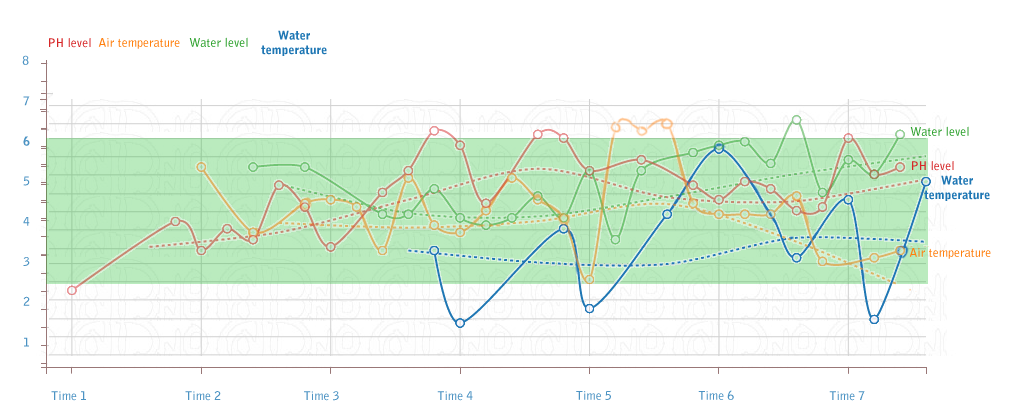
\includegraphics[width=0.9\textwidth]{Mockup}
\caption{Color mockup based on D3.js aesthetics.}
\label{fig:mockup}
\end{figure*}

The next step was to implement a prototype on which we could conduct task-based testing. The prototype was populated with static, generated data, which meant that task performance could be compared a ``correct'' script. The tasks were constructed around ensuring that various features of the interface were easily interpretable (Table~\ref{tab:tasks}). 

\tasktable

Due to lack of availability of ``expert users'' for testing, we adapted the tasks by adding the following scenario preamble.

``You are the manager of an aquaponics farming system. In order to ensure that it is in good working order, you need to monitor the following: pH balance, water temperature, nitrogen levels, air temperature, and dissolved oxygen.  Each of these has boundaries it should stay between for best performance, for example, dissolved oxygen should remain between 30 and 60. If it goes above or below those measurements, the system will need in-person maintenance.''

The feedback from the task-based user testing was then integrated into our final interface. 
 
\subsubsection{Indirect Stakeholders}

The group of indirect stakeholders that we addressed, restaurant customers, constitute a much larger group than the direct stakeholders. Although we were only able to conduct interviews with a very small sample of this group, we were still able to elicit some useful information regarding values. 

Initially, the intent of our investigation was to design an interface that addressed the needs of both direct and indirect stakeholders. The intuition was that the information used by system managers to monitor the operations of the aquaponics system could also be used to assess its sustainability. However, our informal interviews made it clear that the information needs of the indirect stakeholders were too different from those of the direct stakeholders to be addressed by the same interface. Instead of implementing another interface, we decided to present suggestions for how such data could be made available to non-experts interested in sustainability:
\begin{itemize}
\item The live data available to system managers is too much for non-experts to make sense of. Instead, certain system information should be available in summary, e.g., water used annually.
\item In addition to presenting information in summary, data should also be contextualized. Even given data such as annual water use, non-experts are not able to compare to more conventional forms of farming. Suggested contextualization techniques include:
	\begin{itemize}
	\item Resources consumed in system to create a plate of food.
	\item Amount of food that could be produced if the aquaponics system filled a city block. 
	\item Direct comparison to conventional farming methods either inhabiting the same amount of space as the aquaponics system or generating the same amount of food.
	\end{itemize}
\item Ideally, information should be available to restaurant customers in-restaurant. Even restaurant customers who self-reported as being particularly interested in sustainability stated that they would not go out of their way (read, download an app or go to a website) to get sustainability information about food served in restaurants. In order to accomodate this, we suggest a system that generates a data sheet suitable for printing, for the restaurants to carry at their discretion. 
\end{itemize}

\section{Results}

\begin{figure*}
\centering
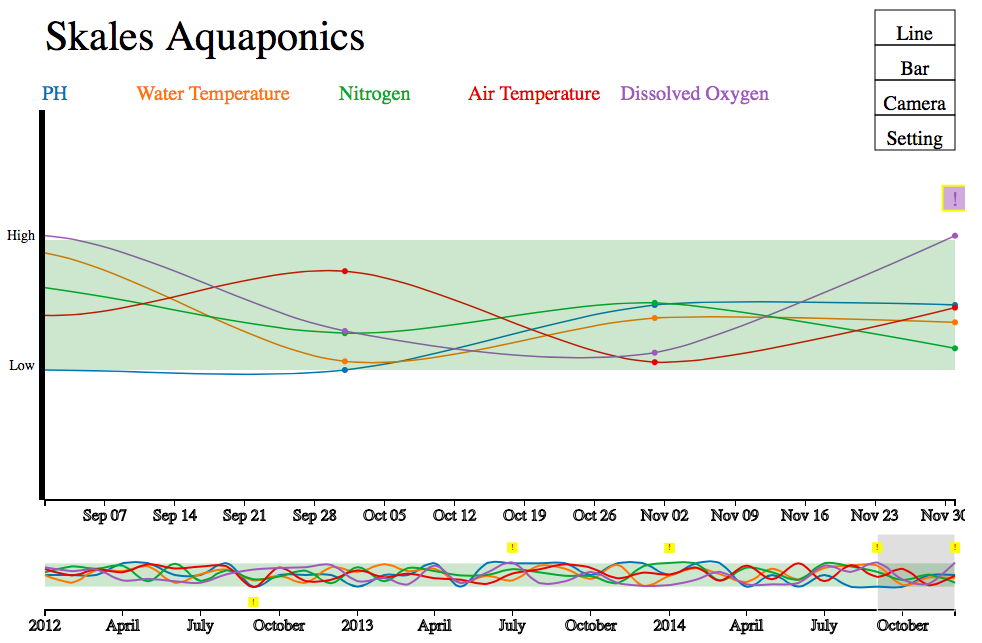
\includegraphics[width=0.9\textwidth]{Visualization_Screenshot}
\caption{Screenshot of the current visualization}
\label{fig:visualization}
\end{figure*}

Our design efforts resulted in a limited \href{http://homes.cs.washington.edu/~samw11/510/}{live prototype}, static version, which can be seen in Figure~\ref{fig:visualization}. 
\footnote{Accessible for the foreseeable future at \url{http://homes.cs.washington.edu/~samw11/510/}} The graph at the top is the trend of the five parameters system managers indicated, i.e., pH value, water temperature, nitrogen, air temperature and dissolved oxygen. The x-axis represents the time and the y-axis represents the value of the those parameters. Color encoding is used in this visualization to represent the parameters. Users can select one of the five parameters at the top and the line of the selected parameter will be highlighted in the graph. 

The green area in the graph represents the safe zone for the parameters. In ideal case, all values should be within the green area. If some of the parameter values venture out of the green area, a little alert box with an exclamation mark on top of the value will appears and the system will alert the user by sending text message, email or even a phone call. In that case, user will able to take action on the problem. The user can also mouse over the points on the line to see the actual value of the parameter at a specific time. A tooltip box will pop up and the background of the tooltip will change to yellow if the value is out of the green area, indicating that there was a problem at that time.

There are more controls at the top right corner. Right now, only the line graph is implemented. The bar graph and the live camera are future work. There is also a settings button so the user can adjust the values for the parameters. For example, the water temperature limits may need to be adjusted depending on the weather. 

There is an overall time graph at the bottom of the visualization. This graph represents all the values from when the system starts running until the present. The main graph at the top shows the time line of the little grey box area at the bottom of the graph. When user moves the grey box, the top graph will change to show the values over the selected time. The width of the grey box can also be changed so that user is not limited to a specific time interval. 

\section{Future Work}
Although the original list of stakeholders was thought to be extensive---including everyone who could conceivably be influenced by the aquaponics system or its interface---an interview with Batya Friedman revealed a particular bias: only humans were considered as stakeholders. The fish living in the aquaponics system, possibly the most direct stakeholder of all, had been overlooked. 

Further development of the alert system would have benefited both the previously-identified stakeholders and the newly-considered ones. By creating a hierarchy of alerts, system managers could be consistently informed about the status of the system, and sufficiently disturbed by an alarm that denotes immediate dangers to the living inhabitants of the aquaponics system. Investigation into the creation and maintenance of such a hierarchy would be an invaluable next step for the success of this interface. 

Our design currently makes strong use of color symbolism. From testing, it was clear that people immediately understood that green means ``good.'' Additional use of color could be used on the graph to show the proximity of parameters to setting off the next tier of alarm, such as ``yellow zones'' and ``red zones'' denoting increasing severity as the parameter deviates farther from its optimal settings.

Another insight Friedman provided was the consideration of how to handle hardware aging. One idea to address aging is to allow system managers to set regularly-recurring maintenance reminders, but more work would need to be done on the form of alert appropriate for such reminders.  

Other extensions to this interface include moving from a passive, monitoring role to being able to actively control certain functions in response to the incoming data, e.g., remotely activating. More visualization could be added such as the bar chat. The live camera could also be added once the hardware is in place. In terms of the alert feature, the system could be adjusted automatically if the value goes off in a small amount rather than keep sending alert to the user.

\section{Conclusion}

We have developed an online interface to aid in the operations of urban aquaponics farming systems. Our design incorporates values of the direct stakeholders (the system managers), which was accomplished using the VSD framework. The features of the system were informed by the opinions of experts that were uncovered through semi-structured interviews and user tests. We were not able to finish all the parts of the project that we originally set out to do, however we made a strong start and collected information that will be useful to future research in this area. As urban farming systems become more important for sustainability in the future, these kinds of interfaces will be necessary to enable ease of operation for a diverse group of food producers.

% Balancing columns in a ref list is a bit of a pain because you
% either use a hack like flushend or balance, or manually insert
% a column break.  http://www.tex.ac.uk/cgi-bin/texfaq2html?label=balance
% multicols doesn't work because we're already in two-column mode,
% and flushend isn't awesome, so I choose balance.  See this
% for more info: http://cs.brown.edu/system/software/latex/doc/balance.pdf
%
% Note that in a perfect world balance wants to be in the first
% column of the last page.
%
% If balance doesn't work for you, you can remove that and
% hard-code a column break into the bbl file right before you
% submit:
%
% http://stackoverflow.com/questions/2149854/how-to-manually-equalize-columns-
% in-an-ieee-paper-if-using-bibtex
%
% Or, just remove \balance and give up on balancing the last page.
%
\balance

\bibliographystyle{acm-sigchi}
\bibliography{FinalProjectReport}

\end{document}
